\documentclass[11pt, class=article, crop=false]{standalone}
\usepackage[subpreambles=true]{standalone}
\usepackage[T1]{fontenc} % for font setting
\usepackage{newtxtext,newtxmath}
\usepackage{import,
            graphicx,
            parskip,
            url,
            amsmath,
            wrapfig,
            fancyhdr,
            soul,
            tabularx,
            authblk,
            textcomp,
            lineno}

% side caption figure
\usepackage{sidecap}
\sidecaptionvpos{figure}{t}

% for special characters in bibliography            
\usepackage[utf8]{inputenc}
\usepackage[T1]{fontenc}

% citation setup
\usepackage[euler]{textgreek}
\usepackage[sort&compress]{natbib}
\setcitestyle{square}
\setcitestyle{comma}
\bibliographystyle{pnas-new}

% caption setup
\usepackage[font={f, small}, labelfont={bf, small}]{caption}
           
% color box
\usepackage[most]{tcolorbox}
\tcbuselibrary{breakable}

% margin
\usepackage[top=2.54cm, bottom=2.54cm, left=2.54cm, right=2.54cm]{geometry}%set margin

% put S before table and figure numbers
\renewcommand{\thetable}{S\arabic{table}}
\renewcommand{\thefigure}{S\arabic{figure}}

% title
\title{Supporting Information for:\\Restoration of aquatic habitat complex extends the foraging window of terrestrial consumers}
\date{} % remove date from title
\author{}

% % author list
% \author[1, a]{Mason Ibrahim}
% \author[2]{Radmila Petric}
% \author[1, b]{Charles F. Wahl}
% \author[1, *]{Akira Terui}

% \affil[1]{Department of Biology, University of North Carolina at Greensboro}
% \affil[2]{Institute for the Environment, University of North Carolina at Chapell Hill}
% \affil[a]{Current Affiliation: Nicholas School of the Environment, Duke University}
% \affil[b]{Current Affiliation: Colorado Water Science Center, U. S. Geological Survey}
% \affil[*]{Corresponding Author: hanabi0111\@gmail.com}

\begin{document}

\maketitle

\section*{Bat Species Composition}

We recorded bat activities at four sites (see Maintext).
Based on previous studies, the following seven species are found in Greensboro: \textit{Eptesicus fuscus} (Big brown bat), \textit{Lasiurus borealis} (Eastern red bat), \textit{Lasiurus cinereus} (Hoary bat), \textit{Lasionycteris noctivagans} (Silver haired bat), \textit{Nycticeius humeralis} (Evening bat), \textit{Perimyotis subflavus} (Tricolored bat), and \textit{Tadarida brasiliensis} (Mexican free-tailed bat).
A bat pass was defined as a recording that included a minimum of three complete bat echolocation call pulses within 0.5 seconds.
Additionally, we used the bat pass match ratio of 0.60 or greater to accept the species identification.

\begin{table}[ht]
\centering
\caption{Summary of bat activity in the study area.
             Total number of bat passes recorded from January 1 to December 31, 2021,
             aggregated by closed and open areas.} 
\label{tab:bat-tbl}
\begingroup\small
\begin{tabular}{llcc}
  \hline
Area & Species & Count & Proportion \\ 
  \hline
Closed & \textit{Eptesicus fuscus} & 7255 & 0.46 \\ 
   & No ID & 4231 & 0.27 \\ 
   & \textit{Nycticeius humeralis} & 1361 & 0.09 \\ 
   & \textit{Lasiurus borealis} & 1062 & 0.07 \\ 
   & \textit{Lasionycteris noctivagans} & 930 & 0.06 \\ 
   & \textit{Lasiurus cinereus} & 459 & 0.03 \\ 
   & \textit{Tadarida brasiliensis} & 384 & 0.02 \\ 
   & \textit{Perimyotis subflavus} & 139 & 0.01 \\ 
  Open & \textit{Eptesicus fuscus} & 39486 & 0.36 \\ 
   & No ID & 29003 & 0.26 \\ 
   & \textit{Lasiurus borealis} & 12044 & 0.11 \\ 
   & \textit{Nycticeius humeralis} & 11869 & 0.11 \\ 
   & \textit{Lasionycteris noctivagans} & 6417 & 0.06 \\ 
   & \textit{Lasiurus cinereus} & 4883 & 0.04 \\ 
   & \textit{Tadarida brasiliensis} & 4556 & 0.04 \\ 
   & \textit{Perimyotis subflavus} & 1550 & 0.01 \\ 
   \hline
\end{tabular}
\endgroup
\end{table}


\section*{Water Temperature}

We deployed water temperature loggers (HOBO TidbiT v2, HOBO\textregistered) in streams and constructed wetlands at the restored sites.
Water temperature was recorded from April 9, 2021, to March 21, 2023, at 30-minute intervals.
Occasionally, loggers were stolen or dislodged by floods.
The data during those periods are unavailable.

\begin{figure}
    \centering
    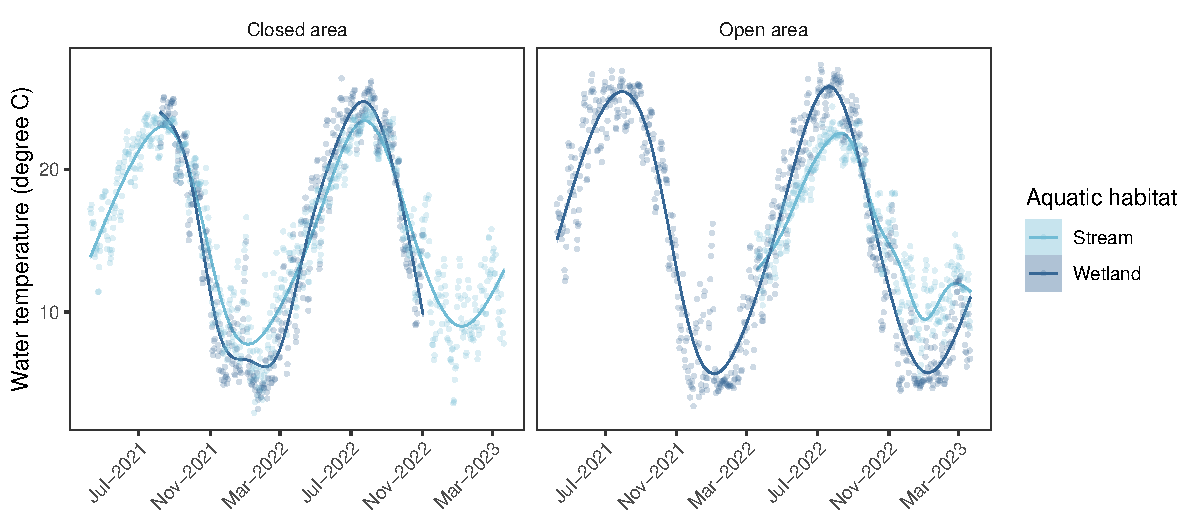
\includegraphics[width=0.95\textwidth]{output/figure_w_temp.pdf}
    \caption{Water temperature trends at restored sites within closed and open areas. Points represent daily average temperatures, with colors distinguishing different aquatic habitats. Solid lines show fitted trends from a Generalized Additive Model applied to temperature data recorded at 30-minute intervals}
    \label{fig:bat-activity}
\end{figure}

% \newpage

% \bibliography{tex/references}

\end{document}